% Options for packages loaded elsewhere
\PassOptionsToPackage{unicode}{hyperref}
\PassOptionsToPackage{hyphens}{url}
%
\documentclass[
]{article}
\usepackage{amsmath,amssymb}
\usepackage{lmodern}
\usepackage{iftex}
\ifPDFTeX
  \usepackage[T1]{fontenc}
  \usepackage[utf8]{inputenc}
  \usepackage{textcomp} % provide euro and other symbols
\else % if luatex or xetex
  \usepackage{unicode-math}
  \defaultfontfeatures{Scale=MatchLowercase}
  \defaultfontfeatures[\rmfamily]{Ligatures=TeX,Scale=1}
\fi
% Use upquote if available, for straight quotes in verbatim environments
\IfFileExists{upquote.sty}{\usepackage{upquote}}{}
\IfFileExists{microtype.sty}{% use microtype if available
  \usepackage[]{microtype}
  \UseMicrotypeSet[protrusion]{basicmath} % disable protrusion for tt fonts
}{}
\makeatletter
\@ifundefined{KOMAClassName}{% if non-KOMA class
  \IfFileExists{parskip.sty}{%
    \usepackage{parskip}
  }{% else
    \setlength{\parindent}{0pt}
    \setlength{\parskip}{6pt plus 2pt minus 1pt}}
}{% if KOMA class
  \KOMAoptions{parskip=half}}
\makeatother
\usepackage{xcolor}
\usepackage[margin=1in]{geometry}
\usepackage{color}
\usepackage{fancyvrb}
\newcommand{\VerbBar}{|}
\newcommand{\VERB}{\Verb[commandchars=\\\{\}]}
\DefineVerbatimEnvironment{Highlighting}{Verbatim}{commandchars=\\\{\}}
% Add ',fontsize=\small' for more characters per line
\usepackage{framed}
\definecolor{shadecolor}{RGB}{248,248,248}
\newenvironment{Shaded}{\begin{snugshade}}{\end{snugshade}}
\newcommand{\AlertTok}[1]{\textcolor[rgb]{0.94,0.16,0.16}{#1}}
\newcommand{\AnnotationTok}[1]{\textcolor[rgb]{0.56,0.35,0.01}{\textbf{\textit{#1}}}}
\newcommand{\AttributeTok}[1]{\textcolor[rgb]{0.77,0.63,0.00}{#1}}
\newcommand{\BaseNTok}[1]{\textcolor[rgb]{0.00,0.00,0.81}{#1}}
\newcommand{\BuiltInTok}[1]{#1}
\newcommand{\CharTok}[1]{\textcolor[rgb]{0.31,0.60,0.02}{#1}}
\newcommand{\CommentTok}[1]{\textcolor[rgb]{0.56,0.35,0.01}{\textit{#1}}}
\newcommand{\CommentVarTok}[1]{\textcolor[rgb]{0.56,0.35,0.01}{\textbf{\textit{#1}}}}
\newcommand{\ConstantTok}[1]{\textcolor[rgb]{0.00,0.00,0.00}{#1}}
\newcommand{\ControlFlowTok}[1]{\textcolor[rgb]{0.13,0.29,0.53}{\textbf{#1}}}
\newcommand{\DataTypeTok}[1]{\textcolor[rgb]{0.13,0.29,0.53}{#1}}
\newcommand{\DecValTok}[1]{\textcolor[rgb]{0.00,0.00,0.81}{#1}}
\newcommand{\DocumentationTok}[1]{\textcolor[rgb]{0.56,0.35,0.01}{\textbf{\textit{#1}}}}
\newcommand{\ErrorTok}[1]{\textcolor[rgb]{0.64,0.00,0.00}{\textbf{#1}}}
\newcommand{\ExtensionTok}[1]{#1}
\newcommand{\FloatTok}[1]{\textcolor[rgb]{0.00,0.00,0.81}{#1}}
\newcommand{\FunctionTok}[1]{\textcolor[rgb]{0.00,0.00,0.00}{#1}}
\newcommand{\ImportTok}[1]{#1}
\newcommand{\InformationTok}[1]{\textcolor[rgb]{0.56,0.35,0.01}{\textbf{\textit{#1}}}}
\newcommand{\KeywordTok}[1]{\textcolor[rgb]{0.13,0.29,0.53}{\textbf{#1}}}
\newcommand{\NormalTok}[1]{#1}
\newcommand{\OperatorTok}[1]{\textcolor[rgb]{0.81,0.36,0.00}{\textbf{#1}}}
\newcommand{\OtherTok}[1]{\textcolor[rgb]{0.56,0.35,0.01}{#1}}
\newcommand{\PreprocessorTok}[1]{\textcolor[rgb]{0.56,0.35,0.01}{\textit{#1}}}
\newcommand{\RegionMarkerTok}[1]{#1}
\newcommand{\SpecialCharTok}[1]{\textcolor[rgb]{0.00,0.00,0.00}{#1}}
\newcommand{\SpecialStringTok}[1]{\textcolor[rgb]{0.31,0.60,0.02}{#1}}
\newcommand{\StringTok}[1]{\textcolor[rgb]{0.31,0.60,0.02}{#1}}
\newcommand{\VariableTok}[1]{\textcolor[rgb]{0.00,0.00,0.00}{#1}}
\newcommand{\VerbatimStringTok}[1]{\textcolor[rgb]{0.31,0.60,0.02}{#1}}
\newcommand{\WarningTok}[1]{\textcolor[rgb]{0.56,0.35,0.01}{\textbf{\textit{#1}}}}
\usepackage{graphicx}
\makeatletter
\def\maxwidth{\ifdim\Gin@nat@width>\linewidth\linewidth\else\Gin@nat@width\fi}
\def\maxheight{\ifdim\Gin@nat@height>\textheight\textheight\else\Gin@nat@height\fi}
\makeatother
% Scale images if necessary, so that they will not overflow the page
% margins by default, and it is still possible to overwrite the defaults
% using explicit options in \includegraphics[width, height, ...]{}
\setkeys{Gin}{width=\maxwidth,height=\maxheight,keepaspectratio}
% Set default figure placement to htbp
\makeatletter
\def\fps@figure{htbp}
\makeatother
\setlength{\emergencystretch}{3em} % prevent overfull lines
\providecommand{\tightlist}{%
  \setlength{\itemsep}{0pt}\setlength{\parskip}{0pt}}
\setcounter{secnumdepth}{-\maxdimen} % remove section numbering
\usepackage{amsmath}
\usepackage{amssymb}
\usepackage{amsthm}
\usepackage{bm}
\ifLuaTeX
  \usepackage{selnolig}  % disable illegal ligatures
\fi
\IfFileExists{bookmark.sty}{\usepackage{bookmark}}{\usepackage{hyperref}}
\IfFileExists{xurl.sty}{\usepackage{xurl}}{} % add URL line breaks if available
\urlstyle{same} % disable monospaced font for URLs
\hypersetup{
  pdftitle={Reporte de estancia},
  pdfauthor={Alejandro Nieto Ramos, Marc Lavielle (asesor)},
  hidelinks,
  pdfcreator={LaTeX via pandoc}}

\title{Reporte de estancia}
\author{Alejandro Nieto Ramos, Marc Lavielle (asesor)}
\date{1 de agosto de 2016}

\begin{document}
\maketitle

\section{El algoritmo EM}\label{EM}

\subsection{El algoritmo EM en general}

Sea \(\bm{Y}\) un vector aleatorio que corresponde con los datos
observados \(\bm{y}\) y cuya función de densidad de probabilidad es
\(g(\bm{y};\bm{\Psi})\), donde \(\bm{\Psi}=(\Psi_1,\ldots,\Psi_d)\) es
un vector de parámetros desconocidos con espacio parametral
\(\bm{\Omega}\).

El algoritmo Esperanza Maximización (\textbf{EM}) permite calcular
estimadores de máxima verosimilitud (\textbf{EML}) a través de un
proceso iterativo, cuando por falta de datos adicionales, la estimación
por máxima verosimilitud sería directa. Desde este punto de vista, al
vector de datos observados \(\bm{y}\) se le considera como incompleto y
a su vez, se toma como una función observable de los datos completos.
Ahora bien, cuando se habla de datos incompletos, no solo se hace
referencia a la falta de datos en sí, sino también a situaciones donde
los datos incompletos representen lo que se podría observar en un
experimento hipotético. En este último contexto, se define a
\(\bm{y_c}\) como el vector de los datos completos y a \(\bm{z}\) como
al vector de los datos adicionales, es decir, los no observables o
faltantes.

Sea entonces \(g_c(\bm{x};\bm{\Psi})\) la función de densidad de
probabilidad del vector aleatorio \(\bm{Y_c}\) que corresponde a los
datos completos. Por lo tanto, la función de verosimilitud de
\(\bm{\Psi}\) si se tuvieran los datos completos, estaría dada por
\(\log L_c(\bm{\Psi})= \log g_c(\bm{y_c};\bm{\Psi})\).

El algoritmo EM resuelve indirectamente el problema de hallar la
solución a la ecuación \begin{equation}
\frac{\partial}{\partial \bm{\Psi}} \log L(\bm{\Psi})=0, \label{MV}
\end{equation} iterando en términos de la función de verosimilitud de
los datos completos \(\log g_c(\bm{y_c})\). Como no se observa, se
cambia por su esperanza condicional dado \(\bm{y}\), usando la
aproximación actual de \(\bm{\Psi}\).

Es decir, sea \(\bm{\Psi}^{(0)}\) un valor inicial de \(\bm{\Psi}\). En
la primera iteración, el paso E requiere del cálculo de
\[ Q( \bm{\Psi};\bm{\Psi}^{(0)})=E_{\bm{\Psi}^{(0)}} [\log L_c(\bm{\Psi})|\bm{y}].\]

El paso M requiere de la maximización de
\(Q( \bm{\Psi};\bm{\Psi}^{(0)})\) con respecto a \(\bm{\Psi}\) sobre el
espacio parametral \(\bm{\Omega}\). Es decir, se toma a
\(\bm{\Psi}^{(1)}\) tal que
\(Q( \bm{\Psi}^{(1)};\bm{\Psi}^{(0)}) \ge Q( \bm{\Psi};\bm{\Psi}^{(0)})\)
para todos los \(\bm{\Psi} \in \bm{\Omega}\). Los pasos E y M se aplican
nuevamente cambiando ahora la aproximación actual por
\(\bm{\Psi}^{(1)}\).

En general, en la iteración \(k+1\), el algoritmo es el siguiente:

\textbf{Paso E.} Se calcula \(Q( \bm{\Psi};\bm{\Psi}^{(k)})\), donde
\(Q( \bm{\Psi};\bm{\Psi}^{(k)})=E_{\bm{\Psi}^{(k)}} [\log L_c(\bm{\Psi})|\bm{y}]\).

\textbf{Paso M.} Se elige \(\bm{\Psi}^{k+1}\) como cualquier valor
\(\bm{\Psi} \in \bm{\Omega}\) que maximice
\(Q( \bm{\Psi};\bm{\Psi}^{(k)})\), es decir,
\(Q( \bm{\Psi}^{(k+1)};\bm{\Psi}^{(k)}) \ge Q( \bm{\Psi};\bm{\Psi}^{(k)})\)
para todo \(\bm{\Psi} \in \bm{\Omega}\). Se alternan repetidamente ambos
pasos hasta que \(|L(\bm{\Psi}^{(k+1)})-L(\bm{\Psi}^{(k)})|<\epsilon\),
para un \(\epsilon>0\) previamente dado, en caso de que la sucesión
\({L(\bm{\Psi})}\) converja. Para asegurar que la sucesión sea
convergente, basta escoger que esté acotada
superiormente\footnote{Teorema de Bolzano.}.

\subsection{El algoritmo EM para modelos de mezclas}

Sea \((Y_1,\ldots,Y_n)\) una muestra aleatoria de tamaño \(n\), donde
\(Y_j\) es un vector de dimensión \(p\) con función de densidad de
probabilidad \(f(y_j)\) en \(\mathbb{R}^p\). Sea
\(\bm{Y}=(Y_1^T,\ldots,Y_n^T)^T\) y defínase una observación de
\(\bm{Y}\) como \(\bm{y}=(y_1^T,\ldots,y_n^T)^T\). Supóngase que que la
densidad \(f(y_j)\) de \(Y_j\) se puede escribir en la forma
\begin{equation}
f(y_j) = \sum_{i=1}^{g} \pi_i \, f_i (y_j),\label{mezcla}
\end{equation} donde las \(f_i\) son las densidades y los valores
\(\pi_i\) son tales que \(\Sigma_{i=1}^{g} \pi_i=1\) con
\(0 \le \pi_i \le 1\) para \(i=1,\ldots,g\).

A las cantidades \(\pi_1,\ldots,\pi_g\) se les conoce como proporciones
de la mezcla o pesos. Dado que las funciones
\(f_1(y_j),\ldots,f_g(y_j)\) son densidades, la ecuación (\ref{mezcla})
define una densidad. A las \(f_i(y_j)\) se les conoce como densidades
componentes de la mezcla. Cabe señalar que en esta formulación, el
número de componentes se considera fijo, aunque en muchas aplicaciones
pueda ser
desconocido.\footnote{En un caso así, el número de componentes se tendría que aproximar.}
A la densidad (\ref{mezcla}) se le conoce como densidad de una mezcla
finita de \(g\) componentes.

\begin{Shaded}
\begin{Highlighting}[]
\NormalTok{mezcla}\OtherTok{\textless{}{-}}\ControlFlowTok{function}\NormalTok{(n,pesos,mu,sigma)}
\NormalTok{\{}
\NormalTok{  G }\OtherTok{\textless{}{-}} \FunctionTok{length}\NormalTok{(mu)}
\NormalTok{  Z }\OtherTok{\textless{}{-}} \FunctionTok{sample}\NormalTok{(}\DecValTok{1}\SpecialCharTok{:}\NormalTok{G, n, }\AttributeTok{prob=}\NormalTok{pesos, }\AttributeTok{replace=}\NormalTok{T)}
\NormalTok{  x}\OtherTok{\textless{}{-}}\ConstantTok{NULL}
  \ControlFlowTok{for}\NormalTok{ (g }\ControlFlowTok{in} \DecValTok{1}\SpecialCharTok{:}\NormalTok{G)}
\NormalTok{  \{}
\NormalTok{    x}\OtherTok{\textless{}{-}}\FunctionTok{c}\NormalTok{(x,}\FunctionTok{rnorm}\NormalTok{(}\FunctionTok{length}\NormalTok{(}\FunctionTok{which}\NormalTok{(Z}\SpecialCharTok{==}\NormalTok{g)),mu[g],sigma[g]))}
\NormalTok{  \}}
  \FunctionTok{return}\NormalTok{(x)}
\NormalTok{\}}
\end{Highlighting}
\end{Shaded}

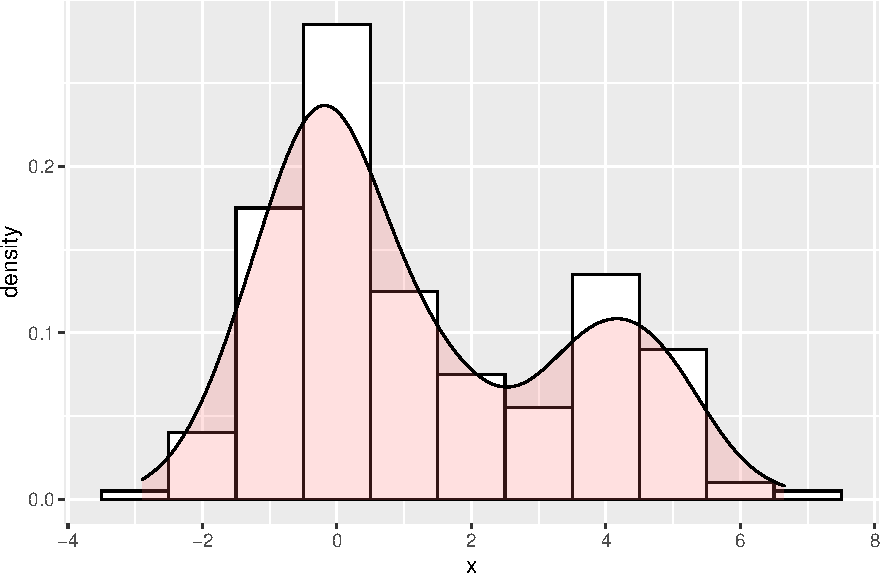
\includegraphics{Reporte0108_files/figure-latex/unnamed-chunk-2-1.pdf}

Gráfica de la mezcla de dos normales, la primera con \(\mu=0,\sigma=1\)
y una proporción del 70\%, y la segunda con \(\mu=4,\sigma=1\) (y una
proporción del 30\%).

\subsubsection{Interpretación}

Una manera clara de generar un vector aleatorio \(Y_{ij}\) con la mezcla
de \(g\) densidades componente \(f(y_j)\) es la siguiente. Defínase a
\(Z_j\) como la variable aleatoria categórica que toma valores en
\(1,\ldots,g\) con probabilidades respectivas \(\pi_1,\ldots,\pi_g\), y
supóngase que la densidad condicional de \(Y_j\) dado \(Z_j=i\) es
\(f_i(y_j)\) para \(i=1,\ldots,g\). Entonces la densidad marginal de
\(Y_j\) está dada por \(f(y_j)\). Considerando este enfoque, la variable
\(Z_j\) se puede pensar como la componente de pertenencia del vector
\(Y_j\). Se define entonces un vector de componentes de pertenencia de
dimensión \(g\), \(\bm{Z_j}\), en lugar de la variable categórica única
\(Z_j\), donde el \(i\)-ésimo elemento de \(\bm{Z_j}\),
\(Z_{ij}=(\bm{Z_j})_i\) es 0 o 1 de acuerdo a si la componente de origen
de \(Y_j\) en la mezcla es igual o no a \(i, \, i=1,\ldots,g\). Por lo
tanto, \(\bm{Z_j}\) se distribuye de acuerdo a una distribución
multinomial que consiste de un experimento en \(g\) categorías con
probabilidades \(\pi_1,\ldots,\pi_g\), es decir,
\(\Pr(\bm{Z_j}=\bm{z_j})=\pi_1^{z_{1j}}\ldots \pi_g^{z_{gj}}\); ésta se
representa como \(Mult_g(1,\bm{\pi})\) donde
\(\bm{\pi}=(\pi_1,\ldots \pi_g)\).

\subsubsection{Enfoque directo}

Sea \begin{equation}
f(y_j;\bm{\Psi})=\sum_{i=1}^{g} \pi_i f_i(y_j;\theta_i)
\end{equation} un modelo de mezcla paramétrico de una muestra aleatoria
observada \(\bm{y}=(y_i^T,\ldots,y_{n}^T)^T\), donde
\(\bm{\Psi}=(\pi_1,\ldots,\pi_{g-1},\xi^T)^T\) es el vector que contiene
todos los parámetros desconocidos de la mezcla del modelo y \(\xi\) es
el vector de los parámetros \(\theta_1,\ldots,\theta_g\) a priori
tomados como distintos. La log verosimilitud de \(\Psi\) que puede
obtenerse de los datos observados está dada por \begin{align}
\log L(\bm{\Psi})&=\sum_{j=1}^n \log(f(y_j;\bm{\Psi}))\\
&=\sum_{j=1}^n \log \left \{ \sum_{i=1}^g \pi_i f_i(y_i;\theta_i) \right \}
\end{align}

Si se calcula el EMV de \(\bm{\Psi}\) tomando esta log verosimilitud, es
preciso resolver
\(\frac{\partial}{\partial \bm{\Psi}} \log L(\bm{\Psi})=0\). Esta
ecuación se puede manipular de modo que el EMV, \(\bm{\hat{\Psi}}\),
satisfaga \begin{equation}
\hat{\pi_i}=\sum_{j=1}^n \frac{1}{n} \,\tau_i(y_j;\bm{\hat{\Psi}})\label{pis},
\end{equation} para todo \(\ i=1,\ldots,g\), y \begin{equation}
\sum_{i=1}^g \sum_{j=1}^n \tau_i(y_j;\bm{\hat{\Psi}}) \frac{\partial}{\partial \xi} \log f_i(y_j;\hat{\theta_i})=0,
\end{equation} donde \begin{equation}
\tau_i (y_j;\bm{\Psi})= \frac{ \pi_i f_i(y_j;\theta_i)}{\sum_{h=1}^{g} \pi_h f_h(y_j;\theta_h)}\label{tau}
\end{equation} es la probabilidad posterior de que \(y_j\) pertenezca a
la componente \(i\) de la mezcla.

\subsubsection{Enfoque donde se ve a los datos como incompletos}

Retómese el mismo enfoque del que se habló en el algoritmo EM, donde el
vector \(\bm{y}=(y_1^T,\ldots,y_n^T)^T\) se toma como incompleto, ya que
los vectores de pertenencia a cierta componente asociados,
\(z_1,\ldots,z_n\), no están disponibles. Con este enfoque, en donde
cada \(y_j\) se ve como que viene de una de los componentes del modelo
de mezcla que se desea ajustar, \(z_j\) es un vector de dimensión \(g\)
con \(z_{ij}=(z_j)_i\) igual a 1 o 0 de de acuerdo a si \(y_j\) vino o
no del componente \(i\)-ésimo de la mezcla, para todo \(i=1,\ldots,g\) y
\(j=1,\ldots,n\). El vector de datos completo es por lo tanto,
\(\bm{y_c}=(y^T,z^T)^T\), donde \(\bm{z}=(z_1^T,\ldots,z_n^T)^T\).

Los vectores de pertenencia a cierta componente \(z_1,\ldots,z_n\) se
toman como realizaciones de los vectores aleatorios \(Z_1,\ldots,Z_n\),
donde por la característica de independencia de los datos, se puede
asumir que se distribuyen independientes con distribución
\(Mult_g(1,\pi)\). Asumir esto significa que la distribución del vector
de los datos completos \(\bm{Y_c}\) da origen a la distribución
apropiada para los datos incompletos \(\bm{Y}\). La log verosimilitud de
los datos completos para \(\bm{\Psi}\), \(\log L_c(\bm{\Psi})\) es
\begin{equation}
\log L_c(\bm{\Psi})=\sum_{i=1}^g \sum_{j=1}^n z_{ij} \{ \log \pi_i+\log f_i(y_j;\theta_i) \} \label{logverosimilitud}.
\end{equation}

\textbf{Paso E}

Se aplica el algoritmo EM a este problema tratando a los \(z_{ij}\) como
datos faltantes. Como la log verosimilitud de los datos completos,
\(L_c\), es lineal con respecto a los datos no observados \(z_{ij}\), el
paso E en la iteración \(k+1\) requiere únicamente del cálculo de la
esperanza condicional actual de \(Z_{ij}\) dados los datos observados
\(y\), donde \(Z_{ij}\) es la variable aleatoria correspondiente a
\(z_{ij}\). Ahora bien, \begin{align}
\mathbb{E}_{ \Psi^{(k)} } ( Z_{ij}|\bm{y} )=& {\Pr}_{\Psi^(k)} (Z_{ij}=1|\bm{y})\\
=& \tau_i(y_j;\bm{\Psi}^{(k)}),
\end{align}

y de acuerdo a la ecuación (\ref{tau}),

\begin{align}
\tau_i( y_j;\bm{\Psi}^{(k)} ) &=
\frac{ \pi_i^{(k)} f_i(y_j;\theta_i^{(k)} )}{f(y_j;\bm{\Psi}^{(k)})}\\
&=\frac{\pi_i^{(k)} f_i( y_j;\theta_i^{(k)})}{\sum_{h=1}^g \pi_h^{(k)} f_h(y_j;\theta_h^{(k)})}
\end{align}

para todo \(i=1,\ldots,g\), \(j=1,\ldots,n\). La cantidad
\(\tau_i(y_j;\bm{\Psi}^{(k)})\) es la probabilidad posterior de que el
\(j\)-ésimo miembro de la muestra con valor observado \(y_j\) pertenezca
al componente \(i\)-ésimo de la mezcla. Aplicando los cálculos hechos en
el párrafo anterior, tomando la esperanza condicional de
(\ref{logverosimilitud}) dado \(y\) se tiene que \begin{equation}
Q(\bm{\Psi};\bm{\Psi}^{(k)})=\sum_{i=1}^{g} \sum_{j=1}^{n} \tau_i(y_j;\bm{\Psi}^{(k)}) \{\log \pi_i + \log f_i(y_j;\theta_i)\}\label{Q}.  
\end{equation}

\textbf{Paso M}

El paso M en la iteración \(k+1\), requiere que se maximice de manera
global \(Q(\bm{\Psi};\bm{\Psi}^{(k)})\) con respecto a \(\bm{\Psi}\)
sobre el espacio parametral \(\bm{\Omega}\) para obtener la estimación
actualizada \(\bm{\Psi}^{(k+1)}\). Para el modelo de mezcla finita, los
estimadores actualizados \(\pi_i^{(k+1)}\) de las proporciones de la
mezcla \(\pi_i\) se calculan independientemente de los estimadores
actualizados \(\xi^{(k+1)}\) del vector de parámetros \(\xi\) que
contiene a los parámetros desconocidos en las densidades componentes.

Si los \(z_{ij}\) fueran observables, entonces el EVM de \(\pi_i\)
estaría dado por la ecuación (\ref{pis}), es decir,
\(\hat{\pi_i}=\sum_{j=1}^{n}\frac{1}{n}z_{ij}\) para \(i=1,\ldots,g\).

Como el paso E solo reemplaza cada \(z_{ij}\) por su esperanza
condicional \(\tau_i(y_j;\bm{\Psi}^{(k)})\) en la log verosimilitud de
los datos completos, el estimador actualizado de \(\pi_i\) está dado al
reemplazar cada \(z_{ij}\) en la ecuación anterior por
\(\tau_i(y_j;\bm{\Psi}^{(k)})\), es decir \begin{equation}
\pi_i^{(k+1)}=\sum_{j=1}^n \frac{1}{n} \, \tau_i(y_j;\bm{\Psi}^{(k)})\label{pi}
\end{equation} para todo \(i=1,\ldots,g\).

Con respecto a la actualización de \(\xi\) en el paso M de la iteración
\(k+1\), se puede ver de la ecuación (\ref{Q}) que \(\xi^{(k+1)}\) se
obtiene como una raíz apropiada de \begin{equation}
\sum_{i=1}^g \sum_{j=1}^n \tau_i(y_j;{\bm{\Psi}}^{(k)}) \frac{\partial}{\partial \xi} \log f_i(y_j;\theta_i)=0,
\end{equation} En ciertos casos, la solución se puede encontrar en forma
analítica, como se verá en la siguiente sección. Finalmente, el
algoritmo termina al igual que como se explicó al final de la sección
\ref{EM}.

\subsection{Mezcla de normales}

Sea ahora \begin{equation}
f(y_j;\bm{\Psi})=\sum_{i=1}^{g}\pi_i \, \phi_i(y_j;\mu_i,\Sigma_i),
\end{equation}

donde
\(\phi(y_j;\mu_i,\Sigma_i)={\frac{1}{{ (\sqrt{2\pi} )}^{n} \sqrt{|\Sigma_i|}}} \exp(-\frac{1}{2}(y_j-\mu_i)^T\Sigma_i^{-1}(y_j-\mu_i))\).

En esta caso, \(\bm{\Psi}=(\pi_1,\dots,\pi_g,\xi^T)^T\), donde \(\xi\)
contiene a los elementos de las componente medias \(\mu_i\) y las
distintas matrices componentes de varianza-covarianza \(\Sigma_i\),
\((i=1,\ldots,g)\).

Se ha visto que en la iteración \(k+1\) del paso E, se reemplazan las
variables de pertenencia a cierta componente, es decir, los \(z_{ij}\),
por sus esperanzas condicionales dadas por sus probabilidades
posteriores de pertenecer a los datos observados \(y_j\),
\(\tau_i(y_j;\Psi^{(k)})\). Por lo tanto,

\begin{equation}
\tau_i( y_j;\bm{\Psi} ) 
=\frac{ \pi_i \, \phi_i( y_j;\mu_i,\Sigma_i)}{\sum_{h=1}^g \pi_h \, \phi_i(y_j;\mu_h,\Sigma_h)}
\end{equation} para \(i=1,\ldots,g\), \(j=1,\ldots,n\).

A continuación se presenta el código en R para calcular \(\tau_i\) en el
caso de una de mezcla de funciones qe se distribuyen normales.

\begin{Shaded}
\begin{Highlighting}[]
\NormalTok{calculotau}\OtherTok{\textless{}{-}}\ControlFlowTok{function}\NormalTok{(x,teta)}
\NormalTok{\{}
\NormalTok{  n}\OtherTok{\textless{}{-}}\FunctionTok{length}\NormalTok{(x)}
\NormalTok{  G}\OtherTok{\textless{}{-}}\FunctionTok{length}\NormalTok{(teta}\SpecialCharTok{$}\NormalTok{p)}
\NormalTok{  tau}\OtherTok{\textless{}{-}}\FunctionTok{matrix}\NormalTok{(}\ConstantTok{NA}\NormalTok{,n,G)}
  \ControlFlowTok{for}\NormalTok{ (g }\ControlFlowTok{in} \DecValTok{1}\SpecialCharTok{:}\NormalTok{G)}
\NormalTok{    tau[,g]}\OtherTok{\textless{}{-}}\NormalTok{teta}\SpecialCharTok{$}\NormalTok{p[g]}\SpecialCharTok{*}\FunctionTok{dnorm}\NormalTok{(x,teta}\SpecialCharTok{$}\NormalTok{mu[g],teta}\SpecialCharTok{$}\NormalTok{sigma[g])}
\NormalTok{  tau}\OtherTok{=}\NormalTok{tau}\SpecialCharTok{/}\FunctionTok{matrix}\NormalTok{(}\FunctionTok{rep}\NormalTok{(}\FunctionTok{rowSums}\NormalTok{(tau),G),}\AttributeTok{nrow=}\NormalTok{n)}
  \FunctionTok{return}\NormalTok{(tau)}
\NormalTok{\}}
\end{Highlighting}
\end{Shaded}

El paso M para componentes normales existe en forma analítica. Las
actualizaciones de las medias componentes \(\mu_i\) y las matrices de
varianza covarianza \(\Sigma_i\) son:

\begin{equation}
\mu_i^{(k+1)}=\frac{\sum_{j=1}^n \tau_{ij}^{(k)}y_j}{\sum_{j=1}^n\tau_{ij}^{(k)}}\label{mu}
\end{equation}

\begin{equation}
\Sigma_i^{(k+1)}=\frac{\sum_{j=1}^n \tau_{ij}^{(k)}(y_j-\mu_i^{(k+1)})(y_j-\mu_i^{(k+1)})^T}{\sum_{j=1}^n \tau_{ij}^{(k)}}\label{sigma}
\end{equation} para \(i=1,\ldots,g\), donde
\(\tau_{ij}^{(k)}=\tau_i(y_j;\Psi^{(k)})\) con \(i=1,\ldots,g\) y
\(j=1,\ldots,n\).

Para simplificar los cálculos computacionales, es conveniente escribir
las actualizaciones anteiores (\ref{mu}) y (\ref{sigma}) en términos de
las esperanzas condicionales actuales de los estadísticos suficientes
\(S_{i1}, S_{12}\) y \(S_{i3}\) para \(\bm{\Psi}\) para el enfoque de
los datos completos. Es decir,
\[ S_{i1}^{(k)}=\sum_{j=1}^{n} \tau_{ij}^{(k)}\]
\[ S_{i2}^{(k)}=\sum_{j=1}^{n} \tau_{ij}^{(k)}y_j\]
\[ S_{i3}^{(k)}=\sum_{j=1}^{n} \tau_{ij}^{(k)}y_j^2.\]

De este modo, el paso E implementado en R queda como sigue:

\begin{Shaded}
\begin{Highlighting}[]
\NormalTok{estadistica}\OtherTok{\textless{}{-}}\ControlFlowTok{function}\NormalTok{(x,Z)}
\NormalTok{\{}
\NormalTok{  G}\OtherTok{\textless{}{-}}\FunctionTok{dim}\NormalTok{(Z)[}\DecValTok{2}\NormalTok{]}
\NormalTok{  M}\OtherTok{\textless{}{-}}\FunctionTok{dim}\NormalTok{(Z)[}\DecValTok{3}\NormalTok{]}
  \ControlFlowTok{if}\NormalTok{ (}\FunctionTok{is.na}\NormalTok{(M))  }
\NormalTok{  \{}
\NormalTok{    M }\OtherTok{\textless{}{-}} \DecValTok{1}
    \FunctionTok{dim}\NormalTok{(Z) }\OtherTok{\textless{}{-}} \FunctionTok{c}\NormalTok{(}\FunctionTok{dim}\NormalTok{(Z),}\DecValTok{1}\NormalTok{)}
\NormalTok{  \}}
\NormalTok{  s1 }\OtherTok{\textless{}{-}} \DecValTok{0}
\NormalTok{  s2 }\OtherTok{\textless{}{-}} \DecValTok{0}
\NormalTok{  s3 }\OtherTok{\textless{}{-}} \DecValTok{0}
  \ControlFlowTok{for}\NormalTok{ (m }\ControlFlowTok{in} \DecValTok{1}\SpecialCharTok{:}\NormalTok{M)}
\NormalTok{  \{}
\NormalTok{    Z.m }\OtherTok{\textless{}{-}}\NormalTok{ Z[,,m]}
\NormalTok{    s1 }\OtherTok{\textless{}{-}}\NormalTok{ s1 }\SpecialCharTok{+} \FunctionTok{colSums}\NormalTok{(Z.m)}
\NormalTok{    s2 }\OtherTok{\textless{}{-}}\NormalTok{ s2 }\SpecialCharTok{+}\NormalTok{ x }\SpecialCharTok{\%*\%}\NormalTok{ Z.m}
\NormalTok{    s3 }\OtherTok{\textless{}{-}}\NormalTok{ s3 }\SpecialCharTok{+}\NormalTok{ (x}\SpecialCharTok{\^{}}\DecValTok{2}\NormalTok{) }\SpecialCharTok{\%*\%}\NormalTok{ Z.m}
\NormalTok{  \}}
\NormalTok{  est}\OtherTok{\textless{}{-}}\FunctionTok{list}\NormalTok{(}\AttributeTok{s1=}\NormalTok{s1}\SpecialCharTok{/}\NormalTok{M,}\AttributeTok{s2=}\NormalTok{s2}\SpecialCharTok{/}\NormalTok{M,}\AttributeTok{s3=}\NormalTok{s3}\SpecialCharTok{/}\NormalTok{M)}
  \FunctionTok{return}\NormalTok{(est)}
\NormalTok{\}}

\NormalTok{pasoE}\OtherTok{\textless{}{-}}\ControlFlowTok{function}\NormalTok{(x,teta)}
\NormalTok{\{}
\NormalTok{  tau }\OtherTok{\textless{}{-}} \FunctionTok{calculotau}\NormalTok{(x,teta)}
\NormalTok{  s }\OtherTok{\textless{}{-}} \FunctionTok{estadistica}\NormalTok{(x,tau)}
  \FunctionTok{return}\NormalTok{(s)}
\NormalTok{\}}
\end{Highlighting}
\end{Shaded}

Ahora bien, el código en R para calcular el paso M es

\begin{Shaded}
\begin{Highlighting}[]
\NormalTok{pasoM}\OtherTok{\textless{}{-}}\ControlFlowTok{function}\NormalTok{(S,n)}
\NormalTok{\{}
\NormalTok{  p}\OtherTok{\textless{}{-}}\NormalTok{S}\SpecialCharTok{$}\NormalTok{s1}\SpecialCharTok{/}\NormalTok{n}
\NormalTok{  mu}\OtherTok{\textless{}{-}}\NormalTok{S}\SpecialCharTok{$}\NormalTok{s2}\SpecialCharTok{/}\NormalTok{S}\SpecialCharTok{$}\NormalTok{s1}
\NormalTok{  sigma}\OtherTok{\textless{}{-}}\FunctionTok{sqrt}\NormalTok{(S}\SpecialCharTok{$}\NormalTok{s3}\SpecialCharTok{/}\NormalTok{S}\SpecialCharTok{$}\NormalTok{s1}\SpecialCharTok{{-}}\NormalTok{(mu)}\SpecialCharTok{\^{}}\DecValTok{2}\NormalTok{)}
\NormalTok{  teta}\OtherTok{\textless{}{-}}\FunctionTok{list}\NormalTok{(}\AttributeTok{p=}\NormalTok{p,}\AttributeTok{mu=}\NormalTok{mu,}\AttributeTok{sigma=}\NormalTok{sigma)}
  \FunctionTok{return}\NormalTok{(teta)}
\NormalTok{\}}
\end{Highlighting}
\end{Shaded}

donde la versoilmilitud está dada por

\begin{Shaded}
\begin{Highlighting}[]
\NormalTok{logLikelihood }\OtherTok{\textless{}{-}} \ControlFlowTok{function}\NormalTok{(x,df)}
\NormalTok{\{}
\NormalTok{  K }\OtherTok{\textless{}{-}} \FunctionTok{dim}\NormalTok{(df)[}\DecValTok{1}\NormalTok{]}
\NormalTok{  G }\OtherTok{\textless{}{-}}\NormalTok{ (}\FunctionTok{dim}\NormalTok{(df)[}\DecValTok{2}\NormalTok{]}\SpecialCharTok{{-}}\DecValTok{1}\NormalTok{)}\SpecialCharTok{/}\DecValTok{3}
\NormalTok{  ll }\OtherTok{\textless{}{-}} \ConstantTok{NULL}
  \ControlFlowTok{for}\NormalTok{ (k }\ControlFlowTok{in}\NormalTok{ (}\DecValTok{1}\SpecialCharTok{:}\NormalTok{K))}
\NormalTok{  \{}
\NormalTok{    lk }\OtherTok{\textless{}{-}} \DecValTok{0}
    \ControlFlowTok{for}\NormalTok{ (g }\ControlFlowTok{in}\NormalTok{ (}\DecValTok{1}\SpecialCharTok{:}\NormalTok{G))}
\NormalTok{    \{}
\NormalTok{      pi.k }\OtherTok{\textless{}{-}}\NormalTok{ df[k,g}\SpecialCharTok{+}\DecValTok{1}\NormalTok{]}
\NormalTok{      mu.k }\OtherTok{\textless{}{-}}\NormalTok{ df[k,G}\SpecialCharTok{+}\NormalTok{g}\SpecialCharTok{+}\DecValTok{1}\NormalTok{]}
\NormalTok{      sigma.k }\OtherTok{\textless{}{-}}\NormalTok{ df[k,}\DecValTok{2}\SpecialCharTok{*}\NormalTok{G}\SpecialCharTok{+}\NormalTok{g}\SpecialCharTok{+}\DecValTok{1}\NormalTok{]}
\NormalTok{      lk }\OtherTok{\textless{}{-}}\NormalTok{ lk }\SpecialCharTok{+}\NormalTok{ pi.k }\SpecialCharTok{*} \FunctionTok{dnorm}\NormalTok{(x, }\AttributeTok{mean=}\NormalTok{mu.k, }\AttributeTok{sd=}\NormalTok{sigma.k)}
\NormalTok{    \}}
\NormalTok{    ll }\OtherTok{\textless{}{-}} \FunctionTok{c}\NormalTok{(ll, }\FunctionTok{sum}\NormalTok{(}\FunctionTok{log}\NormalTok{(lk)))}
\NormalTok{  \}}
\NormalTok{  df}\SpecialCharTok{$}\NormalTok{deviance }\OtherTok{\textless{}{-}} \SpecialCharTok{{-}}\DecValTok{2}\SpecialCharTok{*}\NormalTok{ll}
  \FunctionTok{return}\NormalTok{(df)}
\NormalTok{\}}
\end{Highlighting}
\end{Shaded}

El estimador de la i-ésima proporción \(\pi_i\) está dado por la
ecuación (\ref{pi}).

Finalmente, el programa iterativo que hace uso de las funciones
anteriores se presenta a continuación:

\begin{Shaded}
\begin{Highlighting}[]
\NormalTok{mixt1.em }\OtherTok{\textless{}{-}} \ControlFlowTok{function}\NormalTok{(x, teta0, K)}
\NormalTok{\{}
\NormalTok{  G}\OtherTok{\textless{}{-}}\FunctionTok{length}\NormalTok{(mu)}
\NormalTok{  col.names }\OtherTok{\textless{}{-}} \FunctionTok{c}\NormalTok{(}\StringTok{"iteration"}\NormalTok{, }\FunctionTok{paste0}\NormalTok{(}\StringTok{"p"}\NormalTok{,}\DecValTok{1}\SpecialCharTok{:}\NormalTok{G), }\FunctionTok{paste0}\NormalTok{(}\StringTok{"mu"}\NormalTok{,}\DecValTok{1}\SpecialCharTok{:}\NormalTok{G), }\FunctionTok{paste0}\NormalTok{(}\StringTok{"sigma"}\NormalTok{,}\DecValTok{1}\SpecialCharTok{:}\NormalTok{G))}

\NormalTok{  teta.est }\OtherTok{\textless{}{-}} \FunctionTok{matrix}\NormalTok{(}\ConstantTok{NA}\NormalTok{,K}\SpecialCharTok{+}\DecValTok{1}\NormalTok{,}\DecValTok{3}\SpecialCharTok{*}\NormalTok{G}\SpecialCharTok{+}\DecValTok{1}\NormalTok{)}
\NormalTok{  teta.est[}\DecValTok{1}\NormalTok{,] }\OtherTok{\textless{}{-}} \FunctionTok{c}\NormalTok{(}\DecValTok{0}\NormalTok{, teta0}\SpecialCharTok{$}\NormalTok{p, teta0}\SpecialCharTok{$}\NormalTok{mu, teta0}\SpecialCharTok{$}\NormalTok{sigma)}

\NormalTok{  teta}\OtherTok{\textless{}{-}}\NormalTok{teta0}
  \ControlFlowTok{for}\NormalTok{ (k }\ControlFlowTok{in} \DecValTok{1}\SpecialCharTok{:}\NormalTok{K)}
\NormalTok{  \{}
\NormalTok{    s}\OtherTok{\textless{}{-}}\FunctionTok{pasoE}\NormalTok{(x,teta)}
\NormalTok{    teta}\OtherTok{\textless{}{-}}\FunctionTok{pasoM}\NormalTok{(s,n)}
\NormalTok{    teta.est[k}\SpecialCharTok{+}\DecValTok{1}\NormalTok{,] }\OtherTok{\textless{}{-}} \FunctionTok{c}\NormalTok{(k, teta}\SpecialCharTok{$}\NormalTok{p, teta}\SpecialCharTok{$}\NormalTok{mu, teta}\SpecialCharTok{$}\NormalTok{sigma)}
\NormalTok{  \}}
\NormalTok{  df.em }\OtherTok{\textless{}{-}} \FunctionTok{as.data.frame}\NormalTok{(teta.est)}
  \FunctionTok{names}\NormalTok{(df.em) }\OtherTok{\textless{}{-}}\NormalTok{ col.names}
  \FunctionTok{return}\NormalTok{(df.em)}
\NormalTok{\}}

\CommentTok{\# valores iniciales para el algoritmo}
\NormalTok{pesos0}\OtherTok{\textless{}{-}}\FunctionTok{c}\NormalTok{(.}\DecValTok{5}\NormalTok{,.}\DecValTok{5}\NormalTok{)}
\NormalTok{mu0}\OtherTok{\textless{}{-}}\FunctionTok{c}\NormalTok{(}\DecValTok{1}\NormalTok{,}\DecValTok{2}\NormalTok{)}
\NormalTok{sigma0}\OtherTok{\textless{}{-}}\FunctionTok{c}\NormalTok{(.}\DecValTok{5}\NormalTok{,}\DecValTok{2}\NormalTok{)}

\NormalTok{K }\OtherTok{\textless{}{-}} \DecValTok{250}
\NormalTok{M }\OtherTok{\textless{}{-}} \DecValTok{1}

\NormalTok{G}\OtherTok{\textless{}{-}}\FunctionTok{length}\NormalTok{(mu)}
\NormalTok{col.names }\OtherTok{\textless{}{-}} \FunctionTok{c}\NormalTok{(}\StringTok{"iteration"}\NormalTok{, }\FunctionTok{paste0}\NormalTok{(}\StringTok{"p"}\NormalTok{,}\DecValTok{1}\SpecialCharTok{:}\NormalTok{G), }\FunctionTok{paste0}\NormalTok{(}\StringTok{"mu"}\NormalTok{,}\DecValTok{1}\SpecialCharTok{:}\NormalTok{G), }\FunctionTok{paste0}\NormalTok{(}\StringTok{"sigma"}\NormalTok{,}\DecValTok{1}\SpecialCharTok{:}\NormalTok{G))}
\NormalTok{teta0}\OtherTok{\textless{}{-}}\FunctionTok{list}\NormalTok{(}\AttributeTok{p=}\NormalTok{pesos0,}\AttributeTok{mu=}\NormalTok{mu0,}\AttributeTok{sigma=}\NormalTok{sigma0)}
\NormalTok{s0}\OtherTok{\textless{}{-}}\FunctionTok{list}\NormalTok{(}\AttributeTok{s1=}\DecValTok{0}\NormalTok{,}\AttributeTok{s2=}\DecValTok{0}\NormalTok{,}\AttributeTok{s3=}\DecValTok{0}\NormalTok{)}

\DocumentationTok{\#\#  EM}
\NormalTok{df.em }\OtherTok{\textless{}{-}} \FunctionTok{mixt1.em}\NormalTok{(x, teta0, K)}
\NormalTok{df.em }\OtherTok{\textless{}{-}} \FunctionTok{logLikelihood}\NormalTok{(x,df.em)}
\FunctionTok{print}\NormalTok{(}\FunctionTok{round}\NormalTok{(df.em[}\FunctionTok{nrow}\NormalTok{(df.em),],}\DecValTok{3}\NormalTok{))}
\end{Highlighting}
\end{Shaded}

\begin{verbatim}
##     iteration    p1    p2    mu1   mu2 sigma1 sigma2 deviance
## 251       250 0.692 0.308 -0.046 4.121  1.002  0.921  787.436
\end{verbatim}

\begin{Shaded}
\begin{Highlighting}[]
\NormalTok{graphConvergence }\OtherTok{\textless{}{-}} \ControlFlowTok{function}\NormalTok{(df, }\AttributeTok{title=}\ConstantTok{NULL}\NormalTok{)}
\NormalTok{\{}
\NormalTok{  G }\OtherTok{\textless{}{-}}\NormalTok{ (}\FunctionTok{dim}\NormalTok{(df)[}\DecValTok{2}\NormalTok{]}\SpecialCharTok{{-}}\DecValTok{1}\NormalTok{)}\SpecialCharTok{/}\DecValTok{3}
\NormalTok{  df1}\OtherTok{\textless{}{-}}\FunctionTok{melt}\NormalTok{(df[,}\FunctionTok{c}\NormalTok{(}\DecValTok{1}\NormalTok{,}\DecValTok{2}\NormalTok{,}\DecValTok{3}\NormalTok{)],}\AttributeTok{id.vars=}\StringTok{"iteration"}\NormalTok{,}\AttributeTok{variable=}\StringTok{"proportion"}\NormalTok{)}
\NormalTok{  graf1 }\OtherTok{\textless{}{-}} \FunctionTok{ggplot}\NormalTok{(df1,}\FunctionTok{aes}\NormalTok{(iteration,value))}\SpecialCharTok{+}\FunctionTok{geom\_line}\NormalTok{(}\FunctionTok{aes}\NormalTok{(}\AttributeTok{color=}\NormalTok{proportion))  }\SpecialCharTok{+}
    \FunctionTok{ylab}\NormalTok{(}\StringTok{"proportion"}\NormalTok{) }\SpecialCharTok{+} \FunctionTok{theme}\NormalTok{(}\AttributeTok{legend.position=}\StringTok{"none"}\NormalTok{) }
\NormalTok{  df2}\OtherTok{\textless{}{-}}\FunctionTok{melt}\NormalTok{(df[,}\FunctionTok{c}\NormalTok{(}\DecValTok{1}\NormalTok{,}\DecValTok{4}\NormalTok{,}\DecValTok{5}\NormalTok{)],}\AttributeTok{id.vars=}\StringTok{"iteration"}\NormalTok{,}\AttributeTok{variable=}\StringTok{"mean"}\NormalTok{)}
\NormalTok{  graf2 }\OtherTok{\textless{}{-}} \FunctionTok{ggplot}\NormalTok{(df2,}\FunctionTok{aes}\NormalTok{(iteration,value))}\SpecialCharTok{+}\FunctionTok{geom\_line}\NormalTok{(}\FunctionTok{aes}\NormalTok{(}\AttributeTok{color=}\NormalTok{mean))  }\SpecialCharTok{+}
    \FunctionTok{ylab}\NormalTok{(}\StringTok{"mean"}\NormalTok{) }\SpecialCharTok{+}  \FunctionTok{theme}\NormalTok{(}\AttributeTok{legend.position=}\StringTok{"none"}\NormalTok{) }
\NormalTok{  df3}\OtherTok{\textless{}{-}}\FunctionTok{melt}\NormalTok{(df[,}\FunctionTok{c}\NormalTok{(}\DecValTok{1}\NormalTok{,}\DecValTok{6}\NormalTok{,}\DecValTok{7}\NormalTok{)],}\AttributeTok{id.vars=}\StringTok{"iteration"}\NormalTok{,}\AttributeTok{variable=}\StringTok{"standard.deviation"}\NormalTok{)}
\NormalTok{  graf3 }\OtherTok{\textless{}{-}} \FunctionTok{ggplot}\NormalTok{(df3,}\FunctionTok{aes}\NormalTok{(iteration,value))}\SpecialCharTok{+}\FunctionTok{geom\_line}\NormalTok{(}\FunctionTok{aes}\NormalTok{(}\AttributeTok{color=}\NormalTok{standard.deviation))  }\SpecialCharTok{+}
    \FunctionTok{ylab}\NormalTok{(}\StringTok{"standard.deviation"}\NormalTok{) }\SpecialCharTok{+}  \FunctionTok{theme}\NormalTok{(}\AttributeTok{legend.position=}\StringTok{"none"}\NormalTok{) }
\NormalTok{  graf4 }\OtherTok{\textless{}{-}} \FunctionTok{ggplot}\NormalTok{(df,}\FunctionTok{aes}\NormalTok{(iteration,deviance))}\SpecialCharTok{+}\FunctionTok{geom\_line}\NormalTok{()  }
  \FunctionTok{grid.arrange}\NormalTok{(graf1,graf2,graf3,graf4,}\AttributeTok{nrow=}\DecValTok{2}\NormalTok{, }\AttributeTok{top=}\NormalTok{title)}
\NormalTok{\}}
\FunctionTok{graphConvergence}\NormalTok{(df.em, }\AttributeTok{title=}\StringTok{"EM"}\NormalTok{)}
\end{Highlighting}
\end{Shaded}

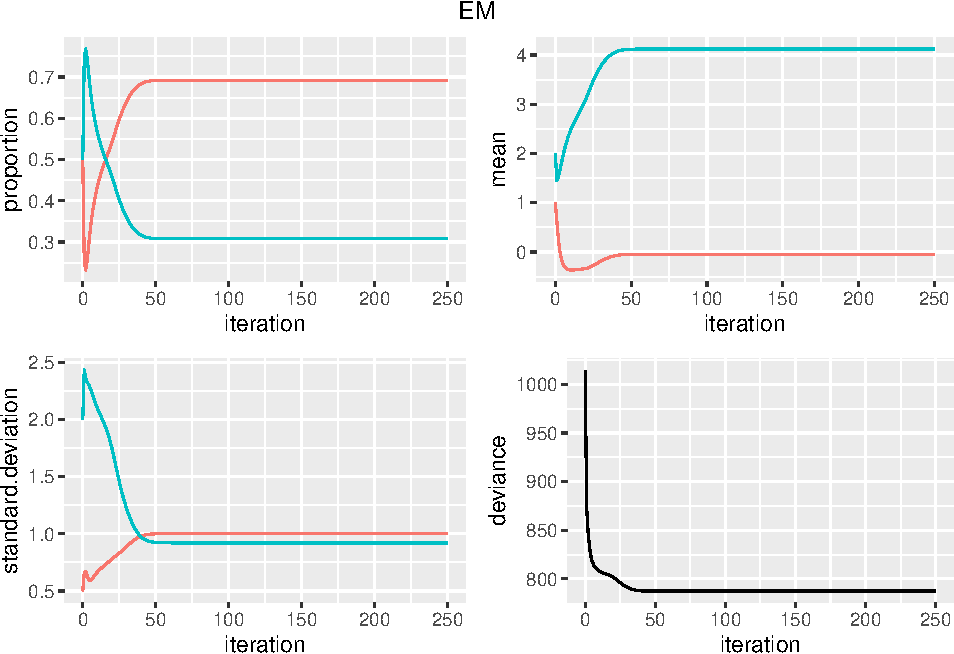
\includegraphics{Reporte0108_files/figure-latex/unnamed-chunk-7-1.pdf}
Ejemplo donde se calculan los parámetros de la mezcla del ejemplo
presentado al principio (\(pesos=(70,30),\mu=(0,4),\sigma=(1,1)\)). Los
valores iniciales dados son \(\pi_0=(.5,.5),\mu=(1,2),\sigma=(.5,2)\)

\section{El algoritmo EM estocástico}

En el paso E del algoritmo EM, cada vector \(z_j\) se reemplaza por su
esperanza condicional dados los datos observados:
\(z_j^{(k)}=(z_{1j}^{(k)},\ldots,z_{gj}^{(k)})^T\), donde
\(z_{ij}^{(k)}\) se define como en la ecuación (\ref{tau}) y es la
probabilidad posterior actual de que la \(j\)-ésima observación venga
del componente \(i\)-ésimo de la mezcla \((i=1,\ldots,g;j=1,\ldots,n)\).
Existen varias versiones del algoritmo EM estocático y se verán dos de
ellas en este documento.

\subsection{El algoritmo EM estocástico de Monte Carlo (MCEM)}

Para este caso, la probabilidad posterior actual se usa en un paso
estocástico E, donde se obtiene una sola
muestra\footnote{Se pueden obtener varias, y de hecho, en el algoritmo programado para este documento, se tiene esta opción.}
de la distribución condicional actual de \(z\) dados los datos
observados \(y\). Por la independencia de los datos completos, esto se
lleva a cabo obteniendo una muestra para cada \(j\) con
\(j=1,\ldots,n\); es decir, se obtiene una muestra \(z_j^{(1_k)}\) de
una distribución multinomial con \(g\) categorías que tienen
probabilidad \(z_{ij}^{(k)}\).

El paso M consiste en encontrar el EMV de \(\bm{\Psi}\) como si los
\(y_1,\ldots,y_n\) fueran clasificados de manera determinista de acuerdo
a \(z_1^{(1_k)},\ldots,z_n^{(1_k)}\).

En resumen, el algoritmo estocástico empieza con probabilidades
multinomiales arbitrarias \(\tau_{ij}^{(0)}\), con \(i=1,\ldots,g\),
para cada observación \(j\). Luego, si \(\bm{\Psi}^{(k)}\) es el valor
de \(\bm{\Psi}\) en la iteración \(k\), se llevan a cabo los siguientes
pasos:

\textbf{Paso estocástico E}.

Para cada \(j\), se obtiene una
muestra\footnote{Éste es un caso particular del algoritmo EM de Monte Carlo, en el cual, se obtienen $M$ muestras y la función $Q$ se aproxima por medio de la suma  $Q(\bm{\Psi},\bm{\Psi}^{(k)})=\frac{1}{M} \sum_{m=1}^{M} \log p(\bm{\Psi} | z^{(m_k)};\bm{y})$.}
de la distribución multinomial con probabilidades \(\tau_{ij}^{(k)}\)
con \(i=1,\ldots,g\), las cuales pueden ser arbitrarias cuando \(k=0\)
(por simplicidad, se pueden tomar todas iguales) o están dadas por el
paso M previo cuando \(k>0\). En la \(k\)-ésima iteración, se define
\(z_j^{(1_k)}=(z_1^{(1_k)},\ldots,z_n^{(1_k)})\) la muestra de la
\(j\)-ésima observación \(y_j\). Esto resulta en una partición de las
\(n\) observaciones \(y_1,\ldots,y_n\) con respecto a las \(g\)
componentes de la mezcla, porque para cada \(j\), exactamente una de
estas \(z_{ij}^{(1_k)}\) es 1 y las otras 0.

\textbf{Paso M}.

Calcular \begin{equation}
\pi_i^{(k+1)}=\sum_{j=1}^n \frac{1}{n} \, z_{ij}^{(1_k)}, 
\end{equation} con \(i=1,\ldots,g\).

Si las \(f_i\) son normales de dimensión \(p\), \(\mu_{i}^{(k+1)}\) y
\(\Sigma_i^{(k+1)}\) están dadas, respectivamente, por las ecuaciones
(\ref{mu}) y (\ref{sigma}). Las probabilidades posteriores para el paso
E estocástico en la siguiente iteración se actualizan de la siguiente
forma:

\begin{align}
\tau_{ij}^{(k+1)}&=\tau_i(y_j;\bm{\Psi}^{(k+1)})\\
&=\frac{\pi_i^{(k+1)}f_i(y_j;\theta^{(k+1)})}{f(y_j;\bm{\Psi}^{(k+1)})}
\end{align}

para \(i=1,\ldots,g\).

Se presenta el código en R del paso estocástico para el caso de una
mezcla de distribuciones normales escalares:

\begin{Shaded}
\begin{Highlighting}[]
\NormalTok{pasoS}\OtherTok{\textless{}{-}}\ControlFlowTok{function}\NormalTok{(x,teta,M)}
\NormalTok{\{}
\NormalTok{  n}\OtherTok{\textless{}{-}}\FunctionTok{length}\NormalTok{(x)}
\NormalTok{  G}\OtherTok{\textless{}{-}}\FunctionTok{length}\NormalTok{(teta}\SpecialCharTok{$}\NormalTok{p)}
\NormalTok{  Z}\OtherTok{\textless{}{-}}\FunctionTok{array}\NormalTok{(}\ConstantTok{NA}\NormalTok{,}\FunctionTok{c}\NormalTok{(n,G,M))}
\NormalTok{  tau}\OtherTok{\textless{}{-}}\FunctionTok{calculotau}\NormalTok{(x,teta)}
  \ControlFlowTok{for}\NormalTok{ (i }\ControlFlowTok{in} \DecValTok{1}\SpecialCharTok{:}\NormalTok{n)}
\NormalTok{  \{ }
\NormalTok{    Z[i,,]}\OtherTok{\textless{}{-}}\FunctionTok{rmultinom}\NormalTok{(}\AttributeTok{n=}\NormalTok{M,}\AttributeTok{size=}\DecValTok{1}\NormalTok{,}\AttributeTok{prob=}\NormalTok{tau[i,])}
\NormalTok{  \}}
  \ControlFlowTok{if}\NormalTok{ (M}\SpecialCharTok{==}\DecValTok{1}\NormalTok{) Z }\OtherTok{\textless{}{-}}\NormalTok{ Z[,,}\DecValTok{1}\NormalTok{]}
  \FunctionTok{return}\NormalTok{(Z)}
\NormalTok{\}  }
\end{Highlighting}
\end{Shaded}

\subsection{El algoritmo EM de aproximación estocástica (SAEM)}

Como se observó en la sección anterior, el algoritmo de EM de Monte
Carlo reemplaza el paso E por una aproximación de Monte Carlo basada en
un gran número de simulaciones independientes de los parámetros
individuales no observados \(z\). En el algoritmo de EM de aproximación
estocástica (\textbf{SAEM}) se reemplaza el paso E por una aproximación
estocástica basada en una sola simulación de \(z\). Este algoritmo
requiere de un valor inicial \(\theta_0\). En la \(k\)-ésima iteración
se tienen tres pasos: un paso de simulación que llamaremos paso S, un
paso de aproximación estocástica y finalmente el paso M de maximización.

\textbf{Paso S}.

Se obtiene una muestra \(z_i^{(k)}\) de una distribución condicional
\(p(z_i | y_i;\Psi^{(k-1)})\).

\textbf{Paso SA}.

Se actualiza \(Q_{k-1}(\Psi)\) de acuerdo a
\[ Q_k(\Psi)=Q_{k-1}(\Psi)+\gamma_{k}(\log p(z_i | y_i;\Psi)-Q_{k-1}(\Psi)),\]
donde \(\{\gamma_k\}_{k=1}^{\infty}\) es una sucesión decreciente tal
que \(\gamma_k \in \mathbb{R}\) con \(\gamma_1=1\).

\textbf{Paso M}

Se actualiza \(\bm{\Psi}^{(k+1)}\) igual que antes.

Se presenta el código en R para el caso del paso de aproximación
estocástica.

\begin{Shaded}
\begin{Highlighting}[]
\NormalTok{pasoSA}\OtherTok{\textless{}{-}}\ControlFlowTok{function}\NormalTok{(x,Z,s.old,gamma)}
\NormalTok{\{}
\NormalTok{  S}\OtherTok{\textless{}{-}}\FunctionTok{estadistica}\NormalTok{(x,Z)}
\NormalTok{  s11}\OtherTok{\textless{}{-}}\NormalTok{s.old}\SpecialCharTok{$}\NormalTok{s1}\SpecialCharTok{+}\NormalTok{gamma}\SpecialCharTok{*}\NormalTok{(S}\SpecialCharTok{$}\NormalTok{s1}\SpecialCharTok{{-}}\NormalTok{s.old}\SpecialCharTok{$}\NormalTok{s1)}
\NormalTok{  s12}\OtherTok{\textless{}{-}}\NormalTok{s.old}\SpecialCharTok{$}\NormalTok{s2}\SpecialCharTok{+}\NormalTok{gamma}\SpecialCharTok{*}\NormalTok{(S}\SpecialCharTok{$}\NormalTok{s2}\SpecialCharTok{{-}}\NormalTok{s.old}\SpecialCharTok{$}\NormalTok{s2)}
\NormalTok{  s13}\OtherTok{\textless{}{-}}\NormalTok{s.old}\SpecialCharTok{$}\NormalTok{s3}\SpecialCharTok{+}\NormalTok{gamma}\SpecialCharTok{*}\NormalTok{(S}\SpecialCharTok{$}\NormalTok{s3}\SpecialCharTok{{-}}\NormalTok{s.old}\SpecialCharTok{$}\NormalTok{s3)}
\NormalTok{  s.new}\OtherTok{\textless{}{-}}\FunctionTok{list}\NormalTok{(}\AttributeTok{s1=}\NormalTok{s11,}\AttributeTok{s2=}\NormalTok{s12,}\AttributeTok{s3=}\NormalTok{s13)}
  \FunctionTok{return}\NormalTok{(s.new)}
\NormalTok{\}}
\end{Highlighting}
\end{Shaded}

Se tiene entonces el algoritmo SAEM para la mezcla presentada para el
algoritmo determinista, donde
\(\{ \gamma_k \}_{k=1}^{\infty}=\{1 \}_{k=1}^{\infty}\) (es decir, éste
es un algoritmo MCEM puro) y \(M=1\).

\begin{Shaded}
\begin{Highlighting}[]
\NormalTok{mixt1.saem }\OtherTok{\textless{}{-}} \ControlFlowTok{function}\NormalTok{(x, teta0, K, K1, M)}
\NormalTok{\{}
\NormalTok{  G}\OtherTok{\textless{}{-}}\FunctionTok{length}\NormalTok{(mu)}
\NormalTok{  col.names }\OtherTok{\textless{}{-}} \FunctionTok{c}\NormalTok{(}\StringTok{"iteration"}\NormalTok{, }\FunctionTok{paste0}\NormalTok{(}\StringTok{"p"}\NormalTok{,}\DecValTok{1}\SpecialCharTok{:}\NormalTok{G), }\FunctionTok{paste0}\NormalTok{(}\StringTok{"mu"}\NormalTok{,}\DecValTok{1}\SpecialCharTok{:}\NormalTok{G), }\FunctionTok{paste0}\NormalTok{(}\StringTok{"sigma"}\NormalTok{,}\DecValTok{1}\SpecialCharTok{:}\NormalTok{G))}
  
\NormalTok{  K2 }\OtherTok{\textless{}{-}}\NormalTok{ K }\SpecialCharTok{{-}}\NormalTok{ K1}
\NormalTok{  gamma}\OtherTok{\textless{}{-}}\FunctionTok{c}\NormalTok{(}\FunctionTok{rep}\NormalTok{(}\DecValTok{1}\NormalTok{,K1),}\DecValTok{1}\SpecialCharTok{/}\NormalTok{(}\DecValTok{1}\SpecialCharTok{:}\NormalTok{K2))}
  
\NormalTok{  teta.est }\OtherTok{\textless{}{-}} \FunctionTok{matrix}\NormalTok{(}\ConstantTok{NA}\NormalTok{,K}\SpecialCharTok{+}\DecValTok{1}\NormalTok{,}\DecValTok{3}\SpecialCharTok{*}\NormalTok{G}\SpecialCharTok{+}\DecValTok{1}\NormalTok{)}
\NormalTok{  teta.est[}\DecValTok{1}\NormalTok{,] }\OtherTok{\textless{}{-}} \FunctionTok{c}\NormalTok{(}\DecValTok{0}\NormalTok{, teta0}\SpecialCharTok{$}\NormalTok{p, teta0}\SpecialCharTok{$}\NormalTok{mu, teta0}\SpecialCharTok{$}\NormalTok{sigma)}
  
\NormalTok{  teta}\OtherTok{\textless{}{-}}\NormalTok{teta0}
\NormalTok{  s}\OtherTok{\textless{}{-}}\NormalTok{s0}
  \ControlFlowTok{for}\NormalTok{ (k }\ControlFlowTok{in} \DecValTok{1}\SpecialCharTok{:}\NormalTok{K)}
\NormalTok{  \{}
\NormalTok{    Z}\OtherTok{\textless{}{-}}\FunctionTok{pasoS}\NormalTok{(x,teta,M)}
\NormalTok{    s}\OtherTok{\textless{}{-}}\FunctionTok{pasoSA}\NormalTok{(x,Z,s,gamma[k])}
\NormalTok{    teta}\OtherTok{\textless{}{-}}\FunctionTok{pasoM}\NormalTok{(s,n)}
\NormalTok{    teta.est[k}\SpecialCharTok{+}\DecValTok{1}\NormalTok{,] }\OtherTok{\textless{}{-}} \FunctionTok{c}\NormalTok{(k, teta}\SpecialCharTok{$}\NormalTok{p, teta}\SpecialCharTok{$}\NormalTok{mu, teta}\SpecialCharTok{$}\NormalTok{sigma)}
\NormalTok{  \}}
\NormalTok{  df.saem }\OtherTok{\textless{}{-}} \FunctionTok{as.data.frame}\NormalTok{(teta.est)}
  \FunctionTok{names}\NormalTok{(df.saem) }\OtherTok{\textless{}{-}}\NormalTok{ col.names}
  \FunctionTok{return}\NormalTok{(df.saem)}
\NormalTok{\}}

\NormalTok{K }\OtherTok{\textless{}{-}} \DecValTok{250}
\NormalTok{K1 }\OtherTok{\textless{}{-}} \DecValTok{250}
\NormalTok{M }\OtherTok{\textless{}{-}} \DecValTok{1}

\DocumentationTok{\#\#  SAEM}
\NormalTok{df.saem }\OtherTok{\textless{}{-}} \FunctionTok{mixt1.saem}\NormalTok{(x, teta0, K, K1, M)}
\NormalTok{df.saem }\OtherTok{\textless{}{-}} \FunctionTok{logLikelihood}\NormalTok{(x,df.saem)}
\FunctionTok{print}\NormalTok{(}\FunctionTok{round}\NormalTok{(df.saem[}\FunctionTok{nrow}\NormalTok{(df.saem),],}\DecValTok{3}\NormalTok{))}
\end{Highlighting}
\end{Shaded}

\begin{verbatim}
##     iteration   p1   p2   mu1   mu2 sigma1 sigma2 deviance
## 251       250 0.71 0.29 0.011 4.236  1.053  0.814  788.594
\end{verbatim}

\begin{Shaded}
\begin{Highlighting}[]
\FunctionTok{graphConvergence}\NormalTok{(df.saem, }\AttributeTok{title=}\StringTok{"SAEM"}\NormalTok{)}
\end{Highlighting}
\end{Shaded}

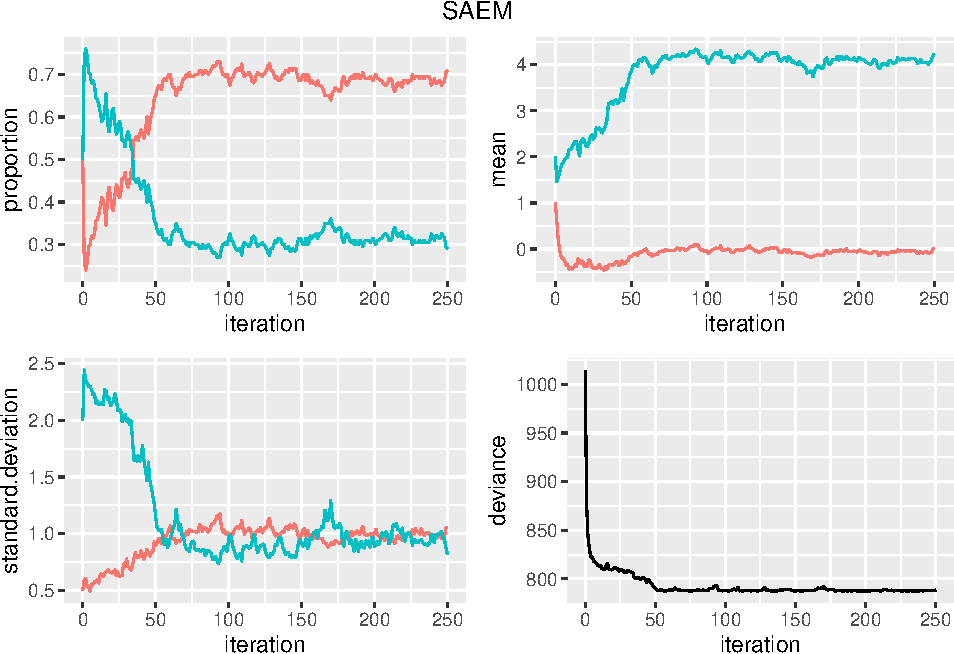
\includegraphics{Reporte0108_files/figure-latex/unnamed-chunk-10-1.pdf}

Haciendo la diferencia entre el método SAEM y EM se tiene:

\begin{Shaded}
\begin{Highlighting}[]
\DocumentationTok{\#\# SAEM {-} EM}
\NormalTok{df.diff }\OtherTok{\textless{}{-}}\NormalTok{ df.saem }\SpecialCharTok{{-}}\NormalTok{ df.em}
\NormalTok{df.diff}\SpecialCharTok{$}\NormalTok{iteration }\OtherTok{\textless{}{-}}\NormalTok{ df.em}\SpecialCharTok{$}\NormalTok{iteration}
\FunctionTok{print}\NormalTok{(}\FunctionTok{round}\NormalTok{(df.diff[}\FunctionTok{nrow}\NormalTok{(df.saem),],}\DecValTok{3}\NormalTok{))}
\end{Highlighting}
\end{Shaded}

\begin{verbatim}
##     iteration    p1     p2   mu1   mu2 sigma1 sigma2 deviance
## 251       250 0.018 -0.018 0.057 0.115   0.05 -0.106    1.159
\end{verbatim}

\begin{Shaded}
\begin{Highlighting}[]
\FunctionTok{graphConvergence}\NormalTok{(df.diff, }\AttributeTok{title=}\StringTok{"SAEM {-} EM"}\NormalTok{)}
\end{Highlighting}
\end{Shaded}

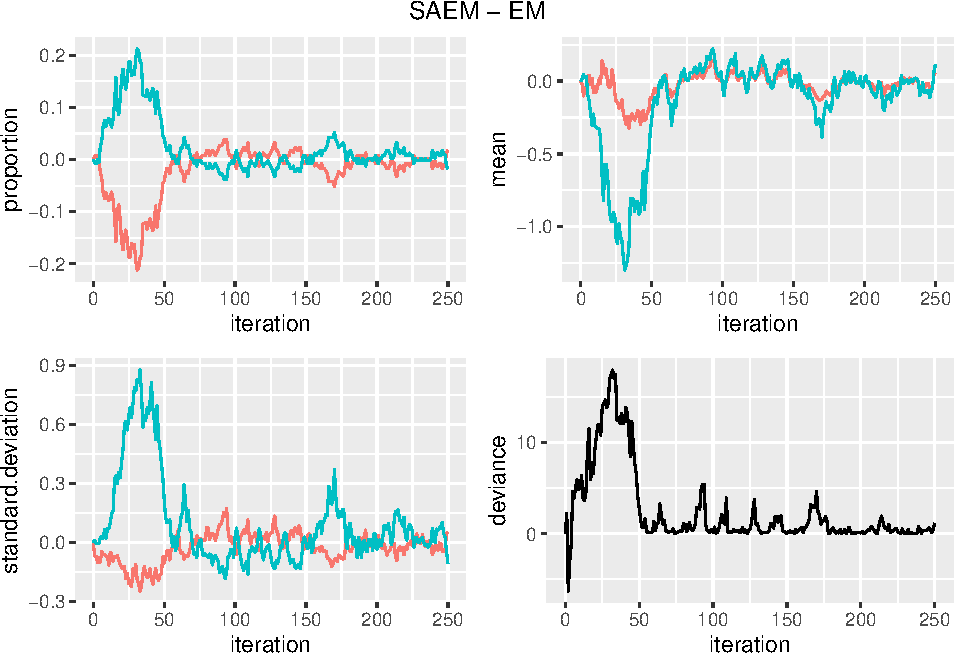
\includegraphics{Reporte0108_files/figure-latex/unnamed-chunk-11-1.pdf}

Si ahora \(M=10\), se puede ver que los valores del algortimo SAEM, el
cual sigue siendo un algoritmo MCEM puro, se aproximan a los del
algoritmo EM (las gráficas de SAEM se suavizan):

\begin{Shaded}
\begin{Highlighting}[]
\NormalTok{K }\OtherTok{\textless{}{-}} \DecValTok{250}
\NormalTok{M }\OtherTok{\textless{}{-}} \DecValTok{10}

\DocumentationTok{\#\#  EM}
\NormalTok{df.em }\OtherTok{\textless{}{-}} \FunctionTok{mixt1.em}\NormalTok{(x, teta0, K)}
\NormalTok{df.em }\OtherTok{\textless{}{-}} \FunctionTok{logLikelihood}\NormalTok{(x,df.em)}

\NormalTok{K }\OtherTok{\textless{}{-}} \DecValTok{250}
\NormalTok{K1 }\OtherTok{\textless{}{-}} \DecValTok{250}
\NormalTok{M }\OtherTok{\textless{}{-}} \DecValTok{10}

\DocumentationTok{\#\#  SAEM}
\NormalTok{df.saem }\OtherTok{\textless{}{-}} \FunctionTok{mixt1.saem}\NormalTok{(x, teta0, K, K1, M)}
\NormalTok{df.saem }\OtherTok{\textless{}{-}} \FunctionTok{logLikelihood}\NormalTok{(x,df.saem)}
\FunctionTok{print}\NormalTok{(}\FunctionTok{round}\NormalTok{(df.saem[}\FunctionTok{nrow}\NormalTok{(df.saem),],}\DecValTok{3}\NormalTok{))}
\end{Highlighting}
\end{Shaded}

\begin{verbatim}
##     iteration    p1   p2    mu1   mu2 sigma1 sigma2 deviance
## 251       250 0.691 0.31 -0.053 4.112  0.994  0.923  787.453
\end{verbatim}

\begin{Shaded}
\begin{Highlighting}[]
\FunctionTok{graphConvergence}\NormalTok{(df.saem, }\AttributeTok{title=}\StringTok{"SAEM"}\NormalTok{)}
\end{Highlighting}
\end{Shaded}

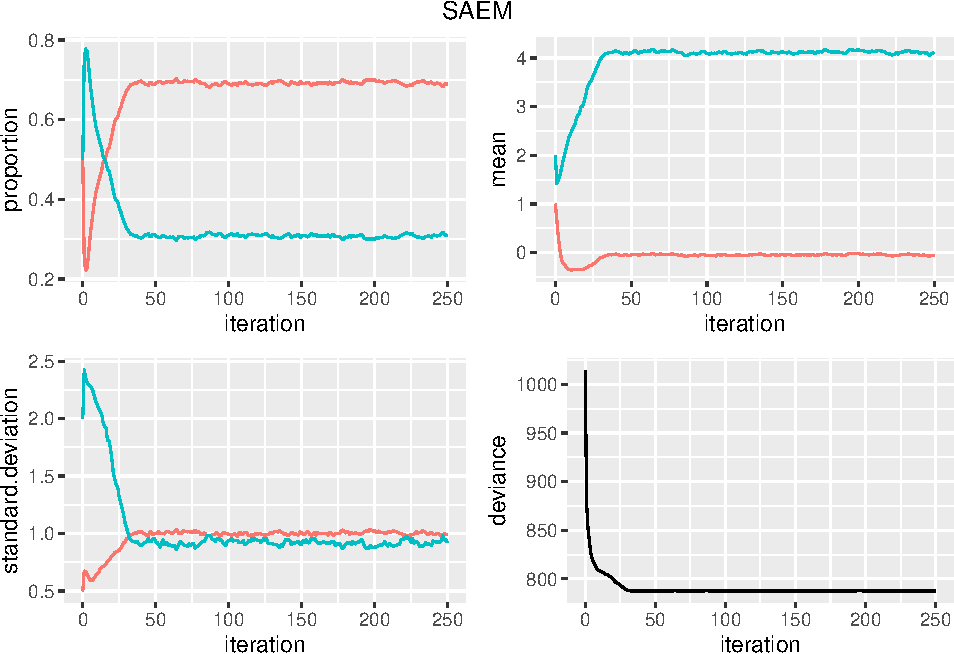
\includegraphics{Reporte0108_files/figure-latex/unnamed-chunk-12-1.pdf}

Si ahora se toma la sucesión decreciente
\(\{ \gamma_k \}_{k=1}^{\infty}=\{\frac{1}{k} \}_{k=1}^{\infty}\), la
gráfica de los valores del algoritmo SAEM se suaviza aún más.

\begin{Shaded}
\begin{Highlighting}[]
\NormalTok{K }\OtherTok{\textless{}{-}} \DecValTok{250}
\NormalTok{M }\OtherTok{\textless{}{-}} \DecValTok{10}

\DocumentationTok{\#\#  EM}
\NormalTok{df.em }\OtherTok{\textless{}{-}} \FunctionTok{mixt1.em}\NormalTok{(x, teta0, K)}
\NormalTok{df.em }\OtherTok{\textless{}{-}} \FunctionTok{logLikelihood}\NormalTok{(x,df.em)}

\NormalTok{K }\OtherTok{\textless{}{-}} \DecValTok{100000}
\NormalTok{K1 }\OtherTok{\textless{}{-}} \DecValTok{0}
\NormalTok{M }\OtherTok{\textless{}{-}} \DecValTok{10}

\DocumentationTok{\#\#  SAEM}
\NormalTok{df.saem }\OtherTok{\textless{}{-}} \FunctionTok{mixt1.saem}\NormalTok{(x, teta0, K, K1, M)}
\NormalTok{df.saem }\OtherTok{\textless{}{-}} \FunctionTok{logLikelihood}\NormalTok{(x,df.saem)}
\FunctionTok{print}\NormalTok{(}\FunctionTok{round}\NormalTok{(df.saem[}\FunctionTok{nrow}\NormalTok{(df.saem),],}\DecValTok{3}\NormalTok{))}
\end{Highlighting}
\end{Shaded}

\begin{verbatim}
##        iteration    p1    p2    mu1 mu2 sigma1 sigma2 deviance
## 100001     1e+05 0.479 0.521 -0.356 2.7  0.713  1.999  805.696
\end{verbatim}

\begin{Shaded}
\begin{Highlighting}[]
\FunctionTok{graphConvergence}\NormalTok{(df.saem, }\AttributeTok{title=}\StringTok{"SAEM"}\NormalTok{)}
\end{Highlighting}
\end{Shaded}

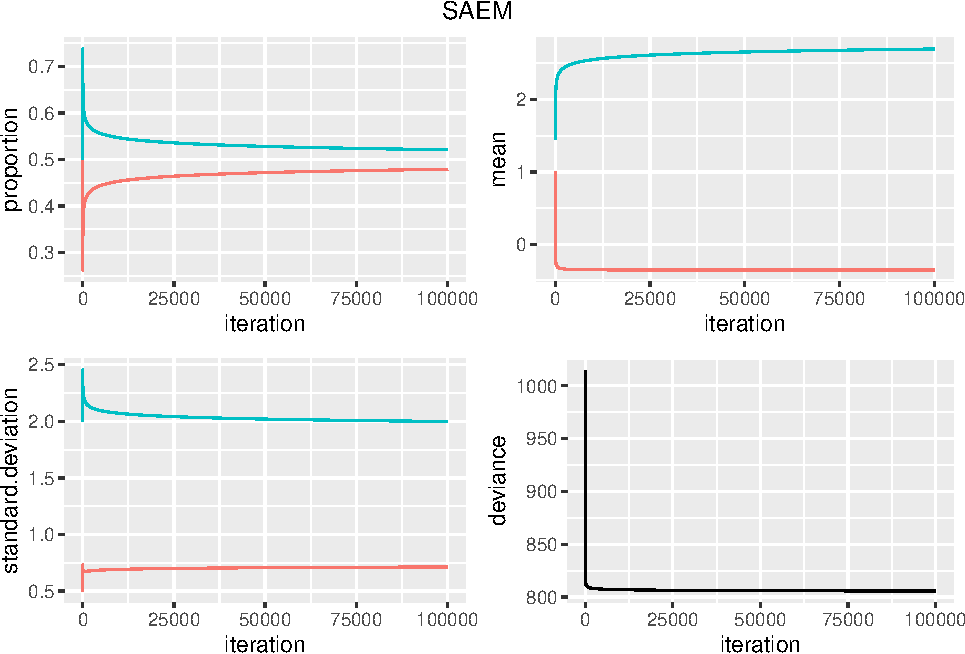
\includegraphics{Reporte0108_files/figure-latex/unnamed-chunk-13-1.pdf}

Lo cierto es que los valores convergen muy lentamente, además de que no
convergen a los valores del algoritmo EM. En este caso entonces, se
puede formar una sucesión para tener una combinación de los algoritmos
MCEM puro y SAEM, para poder encontrar una mejor aproximación al valor
verdadero de los parámetros. Es decir, los primeros \(k_1\) valores de
la sucesión podrían ser todos 1 y a partir del valor del valor \(k_1+1\)
podría tenerse propiamente una sucesión decreciente de números reales.

En el siguiente ejemplo se hace uso de ambos de ambos algortimos
estocásticos con \(k_1\)=100 y
\(\{ \gamma_k \}_{k=1}^{\infty}=\{\frac{1}{k} \}_{k=101}^{\infty}\).

\begin{Shaded}
\begin{Highlighting}[]
\NormalTok{K }\OtherTok{\textless{}{-}} \DecValTok{250}
\NormalTok{K1 }\OtherTok{\textless{}{-}} \DecValTok{100}
\NormalTok{M }\OtherTok{\textless{}{-}} \DecValTok{10}

\DocumentationTok{\#\#  SAEM}
\NormalTok{df.saem }\OtherTok{\textless{}{-}} \FunctionTok{mixt1.saem}\NormalTok{(x, teta0, K, K1, M)}
\NormalTok{df.saem }\OtherTok{\textless{}{-}} \FunctionTok{logLikelihood}\NormalTok{(x,df.saem)}
\FunctionTok{print}\NormalTok{(}\FunctionTok{round}\NormalTok{(df.saem[}\FunctionTok{nrow}\NormalTok{(df.saem),],}\DecValTok{3}\NormalTok{))}
\end{Highlighting}
\end{Shaded}

\begin{verbatim}
##     iteration    p1    p2    mu1   mu2 sigma1 sigma2 deviance
## 251       250 0.691 0.309 -0.049 4.114  0.999  0.927  787.439
\end{verbatim}

\begin{Shaded}
\begin{Highlighting}[]
\FunctionTok{graphConvergence}\NormalTok{(df.saem, }\AttributeTok{title=}\StringTok{"SAEM"}\NormalTok{)}
\end{Highlighting}
\end{Shaded}

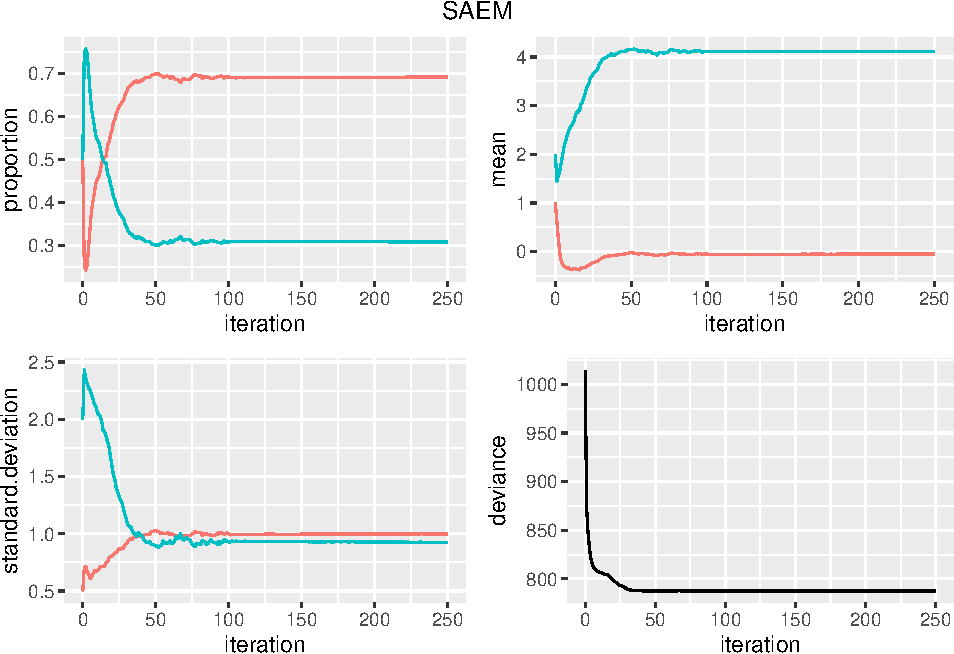
\includegraphics{Reporte0108_files/figure-latex/unnamed-chunk-14-1.pdf}

Por último, se puede modificar el algoritmo SAEM para que en vez de
tomar la sucesión \(\{\gamma_k\}_{k=1}^{\infty}\) se tome la sucesión
\(\{\gamma_k^{\alpha} \}_{k=1}^{\infty}\), donde \(0.5 < \alpha <1\).
Con \(\gamma=.8\) se observa que la aproximación a los valores de los
parámetros es aún mejor, además de que las oscilaciones se vuelven más
pequeñas a medida que se tienen más iteraciones.

\begin{verbatim}
##     iteration    p1    p2    mu1   mu2 sigma1 sigma2 deviance
## 751       750 0.294 0.706 -0.266 4.016    0.8  1.064  786.444
\end{verbatim}

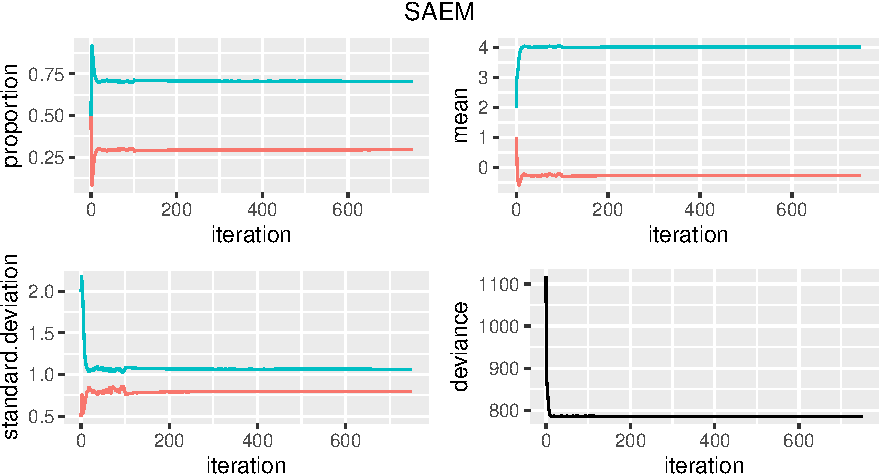
\includegraphics{Reporte0108_files/figure-latex/unnamed-chunk-15-1.pdf}

\begin{verbatim}
##     iteration p1 p2    mu1    mu2 sigma1 sigma2 deviance
## 751       750  0  0 -0.002 -0.001 -0.002  0.002        0
\end{verbatim}

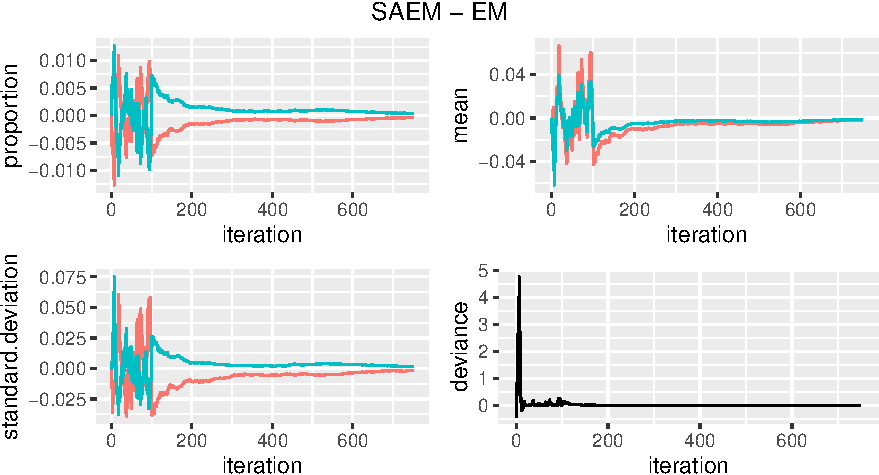
\includegraphics{Reporte0108_files/figure-latex/unnamed-chunk-15-2.pdf}

\begin{thebibliography}{30}

\bibitem{lavielle2014} Lavielle, M. (2014). Mixed effects models for the population approach: models, tasks, methods and tools. CRC press.

\bibitem{McLachlan2000} McLachlan, G. J., \& Peel, D. (2000). Finite Mixture Models. Wiley series in probability and statistics.

\bibitem{McLachlan1997} McLachlan, G. J., \& Krishnan, T. (1997). The EM algorithm and extensions. Wiley series in probability and statistics.

%\bibitem{ribba2012} Ribba, B., Kaloshi, G., Peyre, M., Ricard, D., Calvez, V., Tod, M., ... \& Ducray, F. (2012). A tumor growth inhibition model for low-grade glioma treated with chemotherapy or radiotherapy. Clinical Cancer Research, 18(18), 5071-5080.

\end{thebibliography}

\end{document}
